% Capitolul 2: Seminar - Modele ARMA
% Prezentare academică de calitate Harvard
% Program de licență, Academia de Studii Economice din București

\documentclass[9pt, aspectratio=169, t]{beamer}

% Ensure content fits on slides
\setbeamersize{text margin left=8mm, text margin right=8mm}

%=============================================================================
% THEME AND STYLE CONFIGURATION
%=============================================================================
\usetheme{default}
% Using default theme for clean header/footer control

% Color Palette (matching Redispatch PDF)
\definecolor{MainBlue}{RGB}{26, 58, 110}
\definecolor{AccentBlue}{RGB}{26, 58, 110}
\definecolor{IDAred}{RGB}{205, 0, 0}
\definecolor{DarkGray}{RGB}{51, 51, 51}
\definecolor{MediumGray}{RGB}{128, 128, 128}
\definecolor{LightGray}{RGB}{248, 248, 248}
\definecolor{VeryLightGray}{RGB}{235, 235, 235}
\definecolor{KeynoteGray}{RGB}{218, 218, 218}
\definecolor{SectionGray}{RGB}{120, 120, 120}
\definecolor{FooterGray}{RGB}{100, 100, 100}
\definecolor{Crimson}{RGB}{220, 53, 69}
\definecolor{Forest}{RGB}{46, 125, 50}
\definecolor{Amber}{RGB}{181, 133, 63}
\definecolor{Orange}{RGB}{230, 126, 34}
\definecolor{Purple}{RGB}{142, 68, 173}

% Gradient background (exact Keynote 315° gradient: white to RGB 218,218,218)
\setbeamertemplate{background}{%
    \begin{tikzpicture}[remember picture, overlay]
        \shade[shading=axis, shading angle=315,
        top color=white, bottom color=KeynoteGray]
        (current page.south west) rectangle (current page.north east);
    \end{tikzpicture}%
}
% Fallback solid color for compatibility
\setbeamercolor{background canvas}{bg=}

\setbeamercolor{palette primary}{bg=MainBlue, fg=white}
\setbeamercolor{palette secondary}{bg=MainBlue!85, fg=white}
\setbeamercolor{palette tertiary}{bg=MainBlue!70, fg=white}
\setbeamercolor{structure}{fg=MainBlue}
\setbeamercolor{title}{fg=IDAred}
\setbeamercolor{frametitle}{fg=IDAred, bg=}
\setbeamercolor{block title}{bg=MainBlue, fg=white}
\setbeamercolor{block body}{bg=VeryLightGray, fg=DarkGray}
\setbeamercolor{block title alerted}{bg=Crimson, fg=white}
\setbeamercolor{block body alerted}{bg=Crimson!8, fg=DarkGray}
\setbeamercolor{block title example}{bg=Forest, fg=white}
\setbeamercolor{block body example}{bg=Forest!8, fg=DarkGray}
\setbeamercolor{item}{fg=MainBlue}

% Footer colors (override Madrid theme blue)
\setbeamercolor{author in head/foot}{fg=FooterGray, bg=}
\setbeamercolor{title in head/foot}{fg=FooterGray, bg=}
\setbeamercolor{date in head/foot}{fg=FooterGray, bg=}
\setbeamercolor{section in head/foot}{fg=FooterGray, bg=}
\setbeamercolor{subsection in head/foot}{fg=FooterGray, bg=}

% Bullet styles (apply everywhere including blocks)
\setbeamertemplate{itemize item}{\color{MainBlue}$\boxdot$}
\setbeamertemplate{itemize subitem}{\color{MainBlue}$\blacktriangleright$}
\setbeamertemplate{itemize subsubitem}{\color{MainBlue}\tiny$\bullet$}
\setbeamertemplate{itemize/enumerate body begin}{\normalsize}
\setbeamertemplate{itemize/enumerate subbody begin}{\normalsize}

% Item spacing
\setlength{\leftmargini}{1.5em}
\setlength{\leftmarginii}{1.5em}

\setbeamertemplate{navigation symbols}{}

%=============================================================================
% CUSTOM HEADLINE
%=============================================================================
\setbeamertemplate{headline}{%
    \vskip10pt%
    \hbox to \paperwidth{%
        \hskip0.5cm%
        {\small\color{FooterGray}\renewcommand{\hyperlink}[2]{##2}\insertsectionhead}%
        \hfill%
        \textcolor{FooterGray}{\small\insertframenumber}%
        \hskip0.5cm%
    }%
    \vskip4pt%
    {\color{FooterGray}\hrule height 0.4pt}%
}

%=============================================================================
% CUSTOM FOOTER
%=============================================================================
\usepackage{fontawesome5}

\setbeamertemplate{footline}{%
    {\color{FooterGray}\hrule height 0.4pt}%
    \vskip4pt%
    \hbox to \paperwidth{%
        \hskip0.5cm%
        \textcolor{FooterGray}{\small Analiza și Prognoza Seriilor de Timp}%
        \hfill%
        \raisebox{-0.1em}{%
            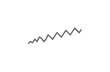
\begin{tikzpicture}[x=0.08em, y=0.08em, line width=0.4pt]
                \draw[FooterGray] (0,3) -- (1,4) -- (2,3.5) -- (3,5) -- (4,4) -- (5,6) -- (6,5.5) -- (7,4) -- (8,5) -- (9,7) -- (10,6) -- (11,5) -- (12,6.5) -- (13,8) -- (14,7) -- (15,6) -- (16,7.5) -- (17,9) -- (18,8) -- (19,7) -- (20,8.5) -- (21,10) -- (22,9) -- (23,8) -- (24,9.5);
            \end{tikzpicture}%
        }%
        \hskip0.5cm%
    }%
    \vskip6pt%
}

%=============================================================================
% PACKAGES
%=============================================================================
\usepackage[utf8]{inputenc}
\usepackage[T1]{fontenc}
\usepackage{amsmath, amssymb, amsthm}
\usepackage{mathtools}
\usepackage{bm}
\usepackage{tikz}
\usetikzlibrary{arrows.meta, positioning, shapes, calc, decorations.pathreplacing, shadings}
\usepackage{booktabs}
\usepackage{multirow}
\usepackage{array}
\usepackage{graphicx}
\usepackage{hyperref}
\usepackage{colortbl}
\hypersetup{colorlinks=true, linkcolor=MainBlue, urlcolor=MainBlue}
\graphicspath{{../logos/}{../charts/}}

%=============================================================================
% CUSTOM COMMANDS
%=============================================================================
\newcommand{\E}{\mathbb{E}}
\newcommand{\Var}{\text{Var}}
\newcommand{\Cov}{\text{Cov}}
\newcommand{\Corr}{\text{Corr}}
\newcommand{\R}{\mathbb{R}}
\newcommand{\RMSE}{\text{RMSE}}
\newcommand{\MAE}{\text{MAE}}
\newcommand{\MAPE}{\text{MAPE}}

% Quiz styling
\newcommand{\correct}{\textcolor{Forest}{\checkmark}}
\newcommand{\incorrect}{\textcolor{Crimson}{\texttimes}}

%=============================================================================
% QUANTLET COMMAND
%=============================================================================
\newcommand{\quantlet}[2]{%
    \hfill\href{#2}{%
        \raisebox{-0.15em}{\includegraphics[height=0.7em]{ql_logo.png}}%
        \textcolor{MainBlue}{\tiny\ #1}%
    }%
}

%=============================================================================
% CUSTOM TITLE PAGE
%=============================================================================
\defbeamertemplate*{title page}{hybrid}[1][]
{
    \vspace{0.2cm}
    % Logos row - top header (with clickable links)
    \begin{center}
        \href{https://www.ase.ro}{\includegraphics[height=1.0cm]{ase_logo.png}}\hspace{0.3cm}%
        \href{https://theida.net}{\includegraphics[height=1.0cm]{ida_logo.png}}\hspace{0.3cm}%
        \href{https://blockchain-research-center.com}{\includegraphics[height=1.0cm]{brc_logo.png}}\hspace{0.3cm}%
        \href{https://www.ai4efin.ase.ro}{\includegraphics[height=1.0cm]{ai4efin_logo.png}}\hspace{0.3cm}%
        \href{https://ipe.ro/new}{\includegraphics[height=1.0cm]{acad_logo.png}}\hspace{0.3cm}%
        \href{https://www.digital-finance-msca.com}{\includegraphics[height=1.0cm]{msca_logo.png}}%
    \end{center}

    \vspace{0.6cm}

    % Main title with Q logos on sides (with clickable links)
    \begin{center}
        \begin{minipage}{0.1\textwidth}
            \centering
            \href{https://quantlet.com}{\includegraphics[height=1.1cm]{ql_logo.png}}
        \end{minipage}%
        \begin{minipage}{0.78\textwidth}
            \centering
            {\LARGE\bfseries\usebeamercolor[fg]{title}\inserttitle}

            \vspace{0.3cm}

            {\usebeamerfont{subtitle}\usebeamercolor[fg]{title}\insertsubtitle}
        \end{minipage}%
        \begin{minipage}{0.1\textwidth}
            \centering
            \href{https://quantinar.com}{\includegraphics[height=1.1cm]{qr_logo.png}}
        \end{minipage}
    \end{center}

    \vspace{0.6cm}

    % Authors (left aligned)
    \hspace{0.5cm}{\usebeamerfont{author}\insertauthor}

    \vspace{0.3cm}

    % Institute/Affiliations (left aligned)
    \hspace{0.5cm}\begin{minipage}[t]{0.9\textwidth}
        \raggedright\small\insertinstitute
    \end{minipage}
}

%=============================================================================
% TITLE INFORMATION
%=============================================================================
\title[Analiza Seriilor de Timp]{Analiza și Prognoza Seriilor de Timp}
\subtitle{Seminar 2: Modele ARMA}
\author[D.T. Pele]{Daniel Traian PELE}
\institute{Academia de Studii Economice din București\\
IDA Institute Digital Assets\\
Blockchain Research Center\\
AI4EFin Artificial Intelligence for Energy Finance\\
Academia Română, Institutul de Prognoză Economică\\
MSCA Digital Finance}
\date{}

\begin{document}

% Title page (no header/footer)
{
\setbeamertemplate{headline}{}
\setbeamertemplate{footline}{}
\begin{frame}
    \titlepage
\end{frame}
}

%=============================================================================
% SEMINAR OUTLINE
%=============================================================================
\section{Prezentare Generală}

\begin{frame}{Cuprins Seminar}
    \textbf{\large Activitățile de Astăzi:}

    \vspace{0.4cm}

    \begin{enumerate}
        \item[\textcolor{MainBlue}{\textbf{1.}}] \textbf{Test Grilă} --- Verificarea înțelegerii conceptelor ARMA
        \vspace{0.15cm}
        \item[\textcolor{MainBlue}{\textbf{2.}}] \textbf{Întrebări Adevărat/Fals} --- Verificări conceptuale
        \vspace{0.15cm}
        \item[\textcolor{MainBlue}{\textbf{3.}}] \textbf{Exerciții de Calcul} --- Practică cu AR/MA
        \vspace{0.15cm}
        \item[\textcolor{MainBlue}{\textbf{4.}}] \textbf{Exerciții Python} --- Ajustare și diagnostice
        \vspace{0.15cm}
        \item[\textcolor{MainBlue}{\textbf{5.}}] \textbf{Întrebări de Discuție} --- Aplicații practice
    \end{enumerate}
\end{frame}

%=============================================================================
% PART 1: MULTIPLE CHOICE QUIZZES
%=============================================================================
\section{Test Grilă}

\begin{frame}{Test 1: Operatorul Lag}
    \begin{alertblock}{Întrebare}
        Care este rezultatul aplicării $(1-L)^2$ lui $X_t$?
    \end{alertblock}

    \vspace{0.5cm}
    \begin{enumerate}[A.]
        \item $X_t - X_{t-1}$
        \item $X_t - 2X_{t-1} + X_{t-2}$
        \item $X_t + X_{t-1} + X_{t-2}$
        \item $X_t - X_{t-2}$
    \end{enumerate}
\end{frame}

\begin{frame}{Test 1: Răspuns}
    \begin{columns}[T]
        \begin{column}{0.52\textwidth}
            \begin{exampleblock}{Răspuns: B}
                $X_t - 2X_{t-1} + X_{t-2}$
            \end{exampleblock}

            \vspace{0.2cm}

            \textbf{Explicație:}
            \begin{align*}
                (1-L)^2 X_t &= (1 - 2L + L^2)X_t \\
                &= X_t - 2X_{t-1} + X_{t-2}
            \end{align*}

            Aceasta este \textbf{diferența de ordinul doi} a lui $X_t$.
        \end{column}
        \begin{column}{0.45\textwidth}
            \includegraphics[width=\textwidth]{ch2_lag_operator.pdf}
            {\tiny Operatorul lag: $L^k X_t = X_{t-k}$}
        \end{column}
    \end{columns}
    \quantlet{TSA\_ch2\_lag\_operator}{https://github.com/QuantLet/TSA/tree/main/TSA\_ch2\_lag\_operator}
\end{frame}

\begin{frame}{Test 2: Staționaritatea AR(1)}
    \begin{alertblock}{Întrebare}
        Pentru ce valoare a lui $\phi$ procesul AR(1) $X_t = 0.5 + \phi X_{t-1} + \varepsilon_t$ este staționar?
    \end{alertblock}

    \vspace{0.5cm}
    \begin{enumerate}[A.]
        \item $\phi = 1.2$
        \item $\phi = 1.0$
        \item $\phi = -0.8$
        \item $\phi = -1.5$
    \end{enumerate}
\end{frame}

\begin{frame}{Test 2: Răspuns}
    \begin{columns}[T]
        \begin{column}{0.52\textwidth}
            \begin{exampleblock}{Răspuns: C}
                $\phi = -0.8$ (Staționar)
            \end{exampleblock}

            \vspace{0.2cm}

            \textbf{Condiția de staționaritate AR(1):}
            $$|\phi| < 1$$

            \vspace{0.2cm}

            Verificarea fiecărei opțiuni:
            \begin{itemize}
                \item A: $|1.2| = 1.2 > 1$ \incorrect
                \item B: $|1.0| = 1$ (rădăcină unitară) \incorrect
                \item C: $|-0.8| = 0.8 < 1$ \correct
                \item D: $|-1.5| = 1.5 > 1$ \incorrect
            \end{itemize}
        \end{column}
        \begin{column}{0.45\textwidth}
            \includegraphics[width=\textwidth]{ch2_ar1.pdf}
            {\tiny AR(1): regiunea staționară $|\phi| < 1$}
        \end{column}
    \end{columns}
    \quantlet{TSA\_ch2\_ar1}{https://github.com/QuantLet/TSA/tree/main/TSA\_ch2\_ar1}
\end{frame}

\begin{frame}{Test 3: Modelul ACF}
    \begin{alertblock}{Întrebare}
        Observați următorul model ACF: vârf semnificativ la lag 1, apoi toate lag-urile în benzile de încredere. PACF arată descreștere graduală. Ce model este sugerat?
    \end{alertblock}

    \vspace{0.5cm}
    \begin{enumerate}[A.]
        \item AR(1)
        \item MA(1)
        \item ARMA(1,1)
        \item Zgomot alb
    \end{enumerate}
\end{frame}

\begin{frame}{Test 3: Răspuns}
    \begin{columns}[T]
        \begin{column}{0.52\textwidth}
            \begin{exampleblock}{Răspuns: B}
                MA(1)
            \end{exampleblock}

            \vspace{0.2cm}

            \textbf{Regula cheie de identificare:}
            \begin{itemize}
                \item ACF se întrerupe după lag $q$ $\Rightarrow$ MA($q$)
                \item PACF se întrerupe după lag $p$ $\Rightarrow$ AR($p$)
            \end{itemize}

            \vspace{0.2cm}

            Aici: ACF se întrerupe la lag 1, PACF descrește

            $\Rightarrow$ \textbf{MA(1)}
        \end{column}
        \begin{column}{0.45\textwidth}
            \includegraphics[width=\textwidth]{ch2_ma1.pdf}
            {\tiny MA(1): ACF se întrerupe după lag 1}
        \end{column}
    \end{columns}
    \quantlet{TSA\_ch2\_ma1}{https://github.com/QuantLet/TSA/tree/main/TSA\_ch2\_ma1}
\end{frame}

\begin{frame}{Test 4: Invertibilitatea MA}
    \begin{alertblock}{Întrebare}
        Pentru procesul MA(1) $X_t = \varepsilon_t + 1.5\varepsilon_{t-1}$, este procesul invertibil?
    \end{alertblock}

    \vspace{0.5cm}
    \begin{enumerate}[A.]
        \item Da, deoarece procesele MA sunt întotdeauna invertibile
        \item Da, deoarece $1.5 > 0$
        \item Nu, deoarece $|\theta| = 1.5 > 1$
        \item Nu, deoarece procesele MA nu sunt niciodată invertibile
    \end{enumerate}
\end{frame}

\begin{frame}{Test 4: Răspuns}
    \begin{columns}[T]
        \begin{column}{0.52\textwidth}
            \begin{exampleblock}{Răspuns: C}
                Nu este invertibil ($|\theta| = 1.5 > 1$)
            \end{exampleblock}

            \vspace{0.2cm}

            \textbf{Invertibilitatea MA(1):}

            Necesită $|\theta| < 1$

            \vspace{0.2cm}

            Echivalent: rădăcina lui $\theta(z) = 1 + \theta z = 0$ trebuie să fie în afara cercului unitate.

            Aici: $z = -1/1.5 = -0.67$ este \textbf{în interior}!

            \vspace{0.2cm}

            $\Rightarrow$ \textcolor{Crimson}{\textbf{Nu este invertibil}}
        \end{column}
        \begin{column}{0.45\textwidth}
            \includegraphics[width=\textwidth]{ch2_ma1.pdf}
            {\tiny Invertibilitate: rădăcina în afara cercului unitate}
        \end{column}
    \end{columns}
    \quantlet{TSA\_ch2\_ma1}{https://github.com/QuantLet/TSA/tree/main/TSA\_ch2\_ma1}
\end{frame}

\begin{frame}{Test 5: Reprezentarea ARMA}
    \begin{alertblock}{Întrebare}
        Forma compactă $\phi(L)X_t = \theta(L)\varepsilon_t$ reprezintă ce model?
    \end{alertblock}

    \vspace{0.5cm}
    \begin{enumerate}[A.]
        \item Model AR pur
        \item Model MA pur
        \item Model ARMA
        \item Niciunul dintre cele de mai sus
    \end{enumerate}
\end{frame}

\begin{frame}{Test 5: Răspuns}
    \begin{columns}[T]
        \begin{column}{0.52\textwidth}
            \begin{exampleblock}{Răspuns: C}
                Model ARMA
            \end{exampleblock}

            \vspace{0.2cm}

            \textbf{Notația cu polinoame lag:}
            \begin{itemize}
                \item $\phi(L) = 1 - \phi_1 L - \cdots - \phi_p L^p$
                \item $\theta(L) = 1 + \theta_1 L + \cdots + \theta_q L^q$
            \end{itemize}

            \vspace{0.2cm}

            Cazuri speciale:
            \begin{itemize}
                \item $\theta(L) = 1$: AR pur
                \item $\phi(L) = 1$: MA pur
            \end{itemize}
        \end{column}
        \begin{column}{0.45\textwidth}
            \includegraphics[width=\textwidth]{ch2_arma.pdf}
            {\tiny ARMA(1,1): combină AR și MA}
        \end{column}
    \end{columns}
    \quantlet{TSA\_ch2\_arma}{https://github.com/QuantLet/TSA/tree/main/TSA\_ch2\_arma}
\end{frame}

\begin{frame}{Test 6: Criterii Informaționale}
    \begin{alertblock}{Întrebare}
        Când comparăm ARMA(1,1) și ARMA(2,1) folosind BIC, care afirmație este corectă?
    \end{alertblock}

    \vspace{0.5cm}
    \begin{enumerate}[A.]
        \item BIC mai mic înseamnă întotdeauna prognoze mai bune
        \item BIC penalizează complexitatea mai puțin decât AIC
        \item Modelul cu BIC mai mic este preferat
        \item BIC poate compara doar modele cu același număr de parametri
    \end{enumerate}
\end{frame}

\begin{frame}{Test 6: Răspuns}
    \begin{columns}[T]
        \begin{column}{0.52\textwidth}
            \begin{exampleblock}{Răspuns: C}
                Modelul cu BIC mai mic este preferat
            \end{exampleblock}

            \vspace{0.2cm}

            \textbf{Criterii Informaționale:}
            \begin{align*}
                \text{AIC} &= -2\ln(\hat{L}) + 2k \\
                \text{BIC} &= -2\ln(\hat{L}) + k\ln(n)
            \end{align*}

            BIC penalizează complexitatea \textbf{mai mult} decât AIC (pentru $n > 7$).

            \vspace{0.2cm}

            $\Rightarrow$ BIC favorizează modele mai simple.
        \end{column}
        \begin{column}{0.45\textwidth}
            \includegraphics[width=\textwidth]{ch2_model_selection.pdf}
            {\tiny Selecția modelului: AIC vs BIC}
        \end{column}
    \end{columns}
    \quantlet{TSA\_ch2\_model\_selection}{https://github.com/QuantLet/TSA/tree/main/TSA\_ch2\_model\_selection}
\end{frame}

\begin{frame}{Test 7: Testul Ljung-Box}
    \begin{alertblock}{Întrebare}
        După ajustarea unui model ARMA(2,1), rulați testul Ljung-Box pe reziduuri și obțineți valoare-p = 0.02. Ce concluzie trageți?
    \end{alertblock}

    \vspace{0.5cm}
    \begin{enumerate}[A.]
        \item Modelul este adecvat
        \item Reziduurile sunt zgomot alb
        \item Există autocorelație semnificativă în reziduuri
        \item Modelul are prea mulți parametri
    \end{enumerate}
\end{frame}

\begin{frame}{Test 7: Răspuns}
    \begin{columns}[T]
        \begin{column}{0.52\textwidth}
            \begin{exampleblock}{Răspuns: C}
                Autocorelație semnificativă în reziduuri
            \end{exampleblock}

            \vspace{0.2cm}

            \textbf{Testul Ljung-Box:}
            \begin{itemize}
                \item $H_0$: Reziduurile sunt zgomot alb
                \item $H_1$: Autocorelație prezentă
            \end{itemize}

            \vspace{0.2cm}

            valoare-p = 0.02 $<$ 0.05

            $\Rightarrow$ \textcolor{Crimson}{\textbf{Respingem $H_0$}}

            Modelul este \textbf{inadecvat} --- încercați alte ordine.
        \end{column}
        \begin{column}{0.45\textwidth}
            \includegraphics[width=\textwidth]{ch2_diagnostics.pdf}
            {\tiny Diagnostice: ACF trebuie să fie zgomot alb}
        \end{column}
    \end{columns}
    \quantlet{TSA\_ch2\_diagnostics}{https://github.com/QuantLet/TSA/tree/main/TSA\_ch2\_diagnostics}
\end{frame}

\begin{frame}{Test 8: Prognoză}
    \begin{alertblock}{Întrebare}
        Pentru un model AR(1) cu $\phi = 0.6$ și medie $\mu = 10$, ce se întâmplă cu prognozele când orizontul $h \to \infty$?
    \end{alertblock}

    \vspace{0.5cm}
    \begin{enumerate}[A.]
        \item Prognozele cresc fără limită
        \item Prognozele converg la 0
        \item Prognozele converg la $\mu = 10$
        \item Prognozele oscilează pentru totdeauna
    \end{enumerate}
\end{frame}

\begin{frame}{Test 8: Răspuns}
    \begin{columns}[T]
        \begin{column}{0.52\textwidth}
            \begin{exampleblock}{Răspuns: C}
                Prognozele converg la $\mu = 10$
            \end{exampleblock}

            \vspace{0.2cm}

            \textbf{Formula de prognoză AR(1):}
            $$\hat{X}_{n+h|n} = \mu + \phi^h(X_n - \mu)$$

            Deoarece $|\phi| = 0.6 < 1$:
            $$\lim_{h \to \infty} \phi^h = 0$$

            $\Rightarrow$ Prognozele converg la $\mu$.

            \textbf{Revenire la medie!}
        \end{column}
        \begin{column}{0.45\textwidth}
            \includegraphics[width=\textwidth]{ch2_forecasting.pdf}
            {\tiny Prognoze AR(1): revenire la medie}
        \end{column}
    \end{columns}
    \quantlet{TSA\_ch2\_forecasting}{https://github.com/QuantLet/TSA/tree/main/TSA\_ch2\_forecasting}
\end{frame}

\begin{frame}{Test 9: Rădăcinile AR(2)}
    \begin{alertblock}{Întrebare}
        Un proces AR(2) are rădăcinile caracteristice $z_1 = 0.8$ și $z_2 = -0.5$. Este staționar?
    \end{alertblock}

    \vspace{0.5cm}
    \begin{enumerate}[A.]
        \item Da, deoarece ambele rădăcini sunt în interiorul cercului unitate
        \item Nu, deoarece o rădăcină este negativă
        \item Nu, deoarece rădăcinile trebuie să fie în afara cercului unitate
        \item Nu se poate determina fără mai multe informații
    \end{enumerate}
\end{frame}

\begin{frame}{Test 9: Răspuns}
    \begin{columns}[T]
        \begin{column}{0.52\textwidth}
            \begin{exampleblock}{Răspuns: C}
                Rădăcinile trebuie să fie în afara cercului unitate
            \end{exampleblock}

            \vspace{0.2cm}

            \textbf{Condiția de staționaritate:}

            Rădăcinile lui $\phi(z) = 0$ trebuie să fie \textbf{în afara} cercului unitate ($|z| > 1$).

            \vspace{0.2cm}

            Aici:
            \begin{itemize}
                \item $|z_1| = 0.8 < 1$ \incorrect
                \item $|z_2| = 0.5 < 1$ \incorrect
            \end{itemize}

            Ambele în interior $\Rightarrow$ \textcolor{Crimson}{\textbf{Nestaționar}}
        \end{column}
        \begin{column}{0.45\textwidth}
            \includegraphics[width=\textwidth]{ch2_ar2.pdf}
            {\tiny AR(2): rădăcini și triunghiul de staționaritate}
        \end{column}
    \end{columns}
    \quantlet{TSA\_ch2\_ar2}{https://github.com/QuantLet/TSA/tree/main/TSA\_ch2\_ar2}
\end{frame}

\begin{frame}{Test 10: Proprietățile MA(q)}
    \begin{alertblock}{Întrebare}
        Pentru un proces MA(2), ACF-ul:
    \end{alertblock}

    \vspace{0.5cm}
    \begin{enumerate}[A.]
        \item Descrește exponențial
        \item Se întrerupe după lag 2
        \item Se întrerupe după lag 1
        \item Nu se întrerupe niciodată
    \end{enumerate}
\end{frame}

\begin{frame}{Test 10: Răspuns}
    \begin{columns}[T]
        \begin{column}{0.52\textwidth}
            \begin{exampleblock}{Răspuns: B}
                Se întrerupe după lag 2
            \end{exampleblock}

            \vspace{0.2cm}

            \textbf{Proprietatea ACF pentru MA($q$):}

            $$\rho(h) = 0 \text{ pentru } h > q$$

            \vspace{0.2cm}

            \begin{itemize}
                \item MA(1): ACF se întrerupe după lag 1
                \item MA(2): ACF se întrerupe după lag 2
                \item MA($q$): ACF se întrerupe după lag $q$
            \end{itemize}

            Caracteristica cheie de identificare!
        \end{column}
        \begin{column}{0.45\textwidth}
            \includegraphics[width=\textwidth]{ch2_ma1.pdf}
            {\tiny MA: întreruperea ACF este semnătura}
        \end{column}
    \end{columns}
    \quantlet{TSA\_ch2\_ma1}{https://github.com/QuantLet/TSA/tree/main/TSA\_ch2\_ma1}
\end{frame}

%=============================================================================
% PART 2: TRUE/FALSE QUESTIONS
%=============================================================================
\section{Întrebări Adevărat/Fals}

\begin{frame}{Adevărat sau Fals? --- Întrebări}
    \footnotesize
    \begin{center}
    \begin{tabular}{p{9cm}c}
        \toprule
        \textbf{Afirmație} & \textbf{A/F?} \\
        \midrule
        1. Un proces AR(2) poate prezenta comportament pseudo-ciclic. & ? \\[0.15cm]
        2. Procesele MA necesită o condiție de staționaritate. & ? \\[0.15cm]
        3. PACF-ul unui proces AR(p) se întrerupe după lag $p$. & ? \\[0.15cm]
        4. Dacă AIC selectează ARMA(2,1) și BIC selectează ARMA(1,1), nu pot fi ambele corecte. & ? \\[0.15cm]
        5. Intervalele de încredere se îngustează pe măsură ce orizontul crește. & ? \\[0.15cm]
        6. Ecuațiile Yule-Walker pot fi folosite pentru a estima parametrii MA. & ? \\
        \bottomrule
    \end{tabular}
    \end{center}
\end{frame}

\begin{frame}{Adevărat sau Fals? --- Răspunsuri}
    \begin{columns}[T]
        \begin{column}{0.55\textwidth}
            \small
            \begin{enumerate}
                \item \textcolor{Forest}{\textbf{ADEVĂRAT}}: AR(2) cu rădăcini complexe $\Rightarrow$ oscilații amortizate
                \vspace{0.1cm}
                \item \textcolor{Crimson}{\textbf{FALS}}: Procesele MA sunt întotdeauna staționare; au nevoie de \textit{invertibilitate}
                \vspace{0.1cm}
                \item \textcolor{Forest}{\textbf{ADEVĂRAT}}: Caracteristica cheie de identificare a AR($p$)
                \vspace{0.1cm}
                \item \textcolor{Crimson}{\textbf{FALS}}: Ambele sunt „corecte" pentru criteriile lor (AIC: estimare, BIC: parsimonie)
                \vspace{0.1cm}
                \item \textcolor{Crimson}{\textbf{FALS}}: IC se \textit{lărgesc} cu orizontul (mai multă incertitudine)
                \vspace{0.1cm}
                \item \textcolor{Crimson}{\textbf{FALS}}: Yule-Walker este pentru AR; MA folosește MLE
            \end{enumerate}
        \end{column}
        \begin{column}{0.42\textwidth}
            \includegraphics[width=\textwidth]{ch2_ar2.pdf}
            {\tiny AR(2): rădăcini complexe $\Rightarrow$ cicluri}
        \end{column}
    \end{columns}
    \quantlet{TSA\_ch2\_ar2}{https://github.com/QuantLet/TSA/tree/main/TSA\_ch2\_ar2}
\end{frame}

%=============================================================================
% PART 3: CALCULATION EXERCISES
%=============================================================================
\section{Exerciții de Calcul}

\begin{frame}{Exercițiul 1: Proprietățile AR(1)}
    \textbf{Problemă:} Considerați procesul AR(1):
    $$X_t = 2 + 0.7 X_{t-1} + \varepsilon_t, \quad \varepsilon_t \sim WN(0, 9)$$

    Calculați:
    \begin{enumerate}
        \item Media $\mu$
        \item Varianța $\gamma(0)$
        \item Autocovarianța $\gamma(1)$ și $\gamma(2)$
        \item Autocorelația $\rho(1)$ și $\rho(2)$
    \end{enumerate}
\end{frame}

\begin{frame}{Exercițiul 1: Soluție}
    \begin{columns}[T]
        \begin{column}{0.52\textwidth}
            Dat: $c = 2$, $\phi = 0.7$, $\sigma^2 = 9$

            \vspace{0.2cm}
            \textbf{1. Media:}
            $$\mu = \frac{c}{1-\phi} = \frac{2}{1-0.7} = \frac{2}{0.3} = \textbf{6.67}$$

            \textbf{2. Varianța:}
            $$\gamma(0) = \frac{\sigma^2}{1-\phi^2} = \frac{9}{1-0.49} = \textbf{17.65}$$

            \textbf{3. Autocovarianța:}
            \begin{align*}
                \gamma(1) &= \phi \cdot \gamma(0) = 0.7 \times 17.65 = \textbf{12.35}\\
                \gamma(2) &= \phi^2 \cdot \gamma(0) = 0.49 \times 17.65 = \textbf{8.65}
            \end{align*}

            \textbf{4. Autocorelația:}
            $$\rho(1) = \phi = \textbf{0.7}, \quad \rho(2) = \phi^2 = \textbf{0.49}$$
        \end{column}
        \begin{column}{0.45\textwidth}
            \includegraphics[width=\textwidth]{ch2_seminar_ex1_ar1.png}
            {\tiny Simulare AR(1) și ACF}
        \end{column}
    \end{columns}
    \quantlet{TSA\_ch2\_ex1\_ar1}{https://github.com/QuantLet/TSA/tree/main/TSA\_ch2\_ex1\_ar1}
\end{frame}

\begin{frame}{Exercițiul 2: Proprietățile MA(1)}
    \textbf{Problemă:} Considerați procesul MA(1):
    $$X_t = 5 + \varepsilon_t - 0.4\varepsilon_{t-1}, \quad \varepsilon_t \sim WN(0, 4)$$

    Calculați:
    \begin{enumerate}
        \item Media $\mu$
        \item Varianța $\gamma(0)$
        \item Autocovarianța $\gamma(1)$
        \item Autocorelația $\rho(1)$
        \item Este acest proces invertibil?
    \end{enumerate}
\end{frame}

\begin{frame}{Exercițiul 2: Soluție}
    \begin{columns}[T]
        \begin{column}{0.52\textwidth}
            Dat: $\mu = 5$, $\theta = -0.4$, $\sigma^2 = 4$

            \vspace{0.2cm}
            \textbf{1. Media:}
            $$\E[X_t] = \mu = \textbf{5}$$

            \textbf{2. Varianța:}
            $$\gamma(0) = \sigma^2(1 + \theta^2) = 4(1.16) = \textbf{4.64}$$

            \textbf{3. Autocovarianța:}
            $$\gamma(1) = \theta\sigma^2 = -0.4 \times 4 = \textbf{-1.6}$$

            \textbf{4. Autocorelația:}
            $$\rho(1) = \frac{\gamma(1)}{\gamma(0)} = \frac{-1.6}{4.64} = \textbf{-0.345}$$

            \textbf{5. Invertibilitate:} $|\theta| = 0.4 < 1$ $\Rightarrow$ \textcolor{Forest}{\textbf{Da}}
        \end{column}
        \begin{column}{0.45\textwidth}
            \includegraphics[width=\textwidth]{ch2_seminar_ex2_ma1.png}
            {\tiny MA(1): ACF se întrerupe după lag 1}
        \end{column}
    \end{columns}
    \quantlet{TSA\_ch2\_ex2\_ma1}{https://github.com/QuantLet/TSA/tree/main/TSA\_ch2\_ex2\_ma1}
\end{frame}

\begin{frame}{Exercițiul 3: Rădăcinile Caracteristice}
    \textbf{Problemă:} Considerați procesul AR(2):
    $$X_t = 0.5X_{t-1} + 0.3X_{t-2} + \varepsilon_t$$

    \begin{enumerate}
        \item Scrieți ecuația caracteristică
        \item Găsiți rădăcinile caracteristice
        \item Este acest proces staționar?
    \end{enumerate}
\end{frame}

\begin{frame}{Exercițiul 3: Soluție}
    \begin{columns}[T]
        \begin{column}{0.52\textwidth}
            \textbf{1. Ecuația caracteristică:}
            $$\phi(z) = 1 - 0.5z - 0.3z^2 = 0$$
            Sau: $0.3z^2 + 0.5z - 1 = 0$

            \vspace{0.2cm}
            \textbf{2. Rădăcinile (formula cuadratică):}
            $$z = \frac{-0.5 \pm \sqrt{0.25 + 1.2}}{0.6}$$
            $$z_1 = \textbf{1.17}, \quad z_2 = \textbf{-2.84}$$

            \vspace{0.2cm}
            \textbf{3. Verificarea staționarității:}

            $|z_1| = 1.17 > 1$ \correct

            $|z_2| = 2.84 > 1$ \correct

            Ambele în afara cercului unitate $\Rightarrow$ \textcolor{Forest}{\textbf{Staționar}}
        \end{column}
        \begin{column}{0.45\textwidth}
            \includegraphics[width=\textwidth]{ch2_seminar_ex3_roots.png}
            {\tiny Rădăcini în afara cercului $\Rightarrow$ staționar}
        \end{column}
    \end{columns}
    \quantlet{TSA\_ch2\_ex3\_roots}{https://github.com/QuantLet/TSA/tree/main/TSA\_ch2\_ex3\_roots}
\end{frame}

\begin{frame}{Exercițiul 4: Prognoză}
    \textbf{Problemă:} Ați ajustat un model AR(1):
    $$X_t = 3 + 0.8X_{t-1} + \varepsilon_t, \quad \sigma^2 = 4$$

    Dat $X_{100} = 20$, calculați:
    \begin{enumerate}
        \item Prognoza la 1 pas înainte $\hat{X}_{101|100}$
        \item Prognoza la 2 pași înainte $\hat{X}_{102|100}$
        \item Prognoza pe termen lung când $h \to \infty$
        \item Intervalul de încredere de 95\% pentru $\hat{X}_{101|100}$
    \end{enumerate}
\end{frame}

\begin{frame}{Exercițiul 4: Soluție}
    \begin{columns}[T]
        \begin{column}{0.52\textwidth}
            Dat: $c = 3$, $\phi = 0.8$, $\sigma^2 = 4$, $X_{100} = 20$

            \textbf{Media:} $\mu = \frac{3}{1-0.8} = \textbf{15}$

            \vspace{0.2cm}
            \textbf{1. Prognoza la un pas:}
            $$\hat{X}_{101|100} = 3 + 0.8 \times 20 = \textbf{19}$$

            \textbf{2. Prognoza la doi pași:}
            $$\hat{X}_{102|100} = 3 + 0.8 \times 19 = \textbf{18.2}$$

            \textbf{3. Prognoza pe termen lung:}
            $$\lim_{h \to \infty} \hat{X}_{100+h|100} = \mu = \textbf{15}$$

            \textbf{4. IC 95\%:}
            $$19 \pm 1.96 \times 2 = \textbf{[15.08, 22.92]}$$
        \end{column}
        \begin{column}{0.45\textwidth}
            \includegraphics[width=\textwidth]{ch2_seminar_ex4_forecast.png}
            {\tiny Prognoza converge la medie}
        \end{column}
    \end{columns}
    \quantlet{TSA\_ch2\_ex4\_forecast}{https://github.com/QuantLet/TSA/tree/main/TSA\_ch2\_ex4\_forecast}
\end{frame}

%=============================================================================
% PART 4: PYTHON EXERCISES
%=============================================================================
\section{Exerciții Python}

\begin{frame}{Exercițiu Python 1: Simulare și Ajustare AR(1)}
    \textbf{Sarcină:}
    \begin{enumerate}
        \item Simulați 300 de observații dintr-un AR(1) cu $\phi = 0.6$
        \item Reprezentați grafic seria și ACF/PACF
        \item Ajustați un model AR(1) și comparați $\hat{\phi}$ vs $\phi$ real
        \item Examinați diagnosticele reziduurilor
    \end{enumerate}

    \vspace{0.3cm}
    \textbf{Cod cheie:}
    \begin{verbatim}
from statsmodels.tsa.arima.model import ARIMA
model = ARIMA(x, order=(1, 0, 0)).fit()
print(model.summary())
    \end{verbatim}

    \quantlet{TSA\_ch2\_python\_simulate}{https://github.com/QuantLet/TSA/tree/main/TSA\_ch2\_python\_simulate}
\end{frame}

\begin{frame}{Exercițiu Python 2: Selecția Modelului}
    \textbf{Sarcină:}
    \begin{enumerate}
        \item Încărcați o serie de timp și verificați staționaritatea (testul ADF)
        \item Comparați AIC/BIC pentru AR(1), MA(1), ARMA(1,1), ARMA(2,1)
        \item Selectați cel mai bun model
        \item Generați prognoze cu intervale de încredere
    \end{enumerate}

    \vspace{0.3cm}
    \textbf{Funcții cheie:}
    \begin{itemize}
        \item \texttt{adfuller(x)} pentru testul de staționaritate
        \item \texttt{model.aic}, \texttt{model.bic} pentru criterii
        \item \texttt{model.get\_forecast(h)} pentru predicții
    \end{itemize}

    \quantlet{TSA\_ch2\_python\_selection}{https://github.com/QuantLet/TSA/tree/main/TSA\_ch2\_python\_selection}
\end{frame}

\begin{frame}{Exercițiu Python 3: Verificarea Diagnosticelor}
    \textbf{Sarcină:} După ajustarea unui model, efectuați diagnostice complete:
    \begin{enumerate}
        \item Reprezentați grafic reziduurile în timp
        \item Reprezentați grafic ACF-ul reziduurilor
        \item Creați graficul Q-Q pentru normalitate
        \item Rulați testul Ljung-Box
    \end{enumerate}

    \vspace{0.3cm}
    \textbf{Funcții cheie:}
    \begin{itemize}
        \item \texttt{model.resid} pentru reziduuri
        \item \texttt{plot\_acf(resid)} pentru graficul ACF
        \item \texttt{stats.probplot(resid)} pentru graficul Q-Q
        \item \texttt{acorr\_ljungbox(resid, lags=[10])} pentru test
    \end{itemize}

    \quantlet{TSA\_ch2\_python\_diagnostics}{https://github.com/QuantLet/TSA/tree/main/TSA\_ch2\_python\_diagnostics}
\end{frame}

%=============================================================================
% PART 5: DISCUSSION QUESTIONS
%=============================================================================
\section{Întrebări de Discuție}

\begin{frame}{Discuție 1: Selecția Modelului}
    \textbf{Scenariu:} Modelați rate de inflație lunare. După verificarea staționarității:
    \begin{itemize}
        \item ACF: semnificativ la lag-urile 1, 2, 3, apoi descrește
        \item PACF: semnificativ la lag-urile 1, 2, apoi se întrerupe
        \item AIC selectează ARMA(2,3)
        \item BIC selectează AR(2)
    \end{itemize}

    \vspace{0.3cm}
    \textbf{Întrebări:}
    \begin{enumerate}
        \item Ce sugerează modelul ACF/PACF?
        \item De ce nu sunt de acord AIC și BIC?
        \item Ce model ați alege și de ce?
        \item Ce verificări suplimentare ați efectua?
    \end{enumerate}
\end{frame}

\begin{frame}{Discuție 2: Evaluarea Prognozei}
    \textbf{Scenariu:} Ajustați un model ARMA(1,1) pe randamente zilnice de acțiuni. Ajustarea în eșantion arată bine (Ljung-Box p = 0.45), dar RMSE în afara eșantionului este mai rău decât mersul aleatoriu.

    \vspace{0.3cm}
    \textbf{Întrebări:}
    \begin{enumerate}
        \item Este aceasta surprinzător? De ce sau de ce nu?
        \item Ce ne spune despre predictibilitatea randamentelor?
        \item Ar trebui să concluzionați că modelul ARMA este inutil?
        \item Ce alternative ați putea considera?
    \end{enumerate}

    \vspace{0.3cm}
    \textbf{Indiciu:} Gândiți-vă la Ipoteza Pieței Eficiente și la ce captează ARMA vs. gruparea volatilității.
\end{frame}

%=============================================================================
% KEY FORMULAS SUMMARY
%=============================================================================
\section{Formule Cheie}

\begin{frame}{Rezumat Formule Cheie}
    \small
    \begin{center}
    \begin{tabular}{ll}
        \toprule
        \textbf{Concept} & \textbf{Formula} \\
        \midrule
        Media AR(1) & $\mu = c/(1-\phi)$ \\[0.1cm]
        Varianța AR(1) & $\gamma(0) = \sigma^2/(1-\phi^2)$ \\[0.1cm]
        ACF AR(1) & $\rho(h) = \phi^h$ \\[0.1cm]
        Staționaritate AR(1) & $|\phi| < 1$ \\[0.1cm]
        \midrule
        Varianța MA(1) & $\gamma(0) = \sigma^2(1+\theta^2)$ \\[0.1cm]
        ACF MA(1) & $\rho(1) = \theta/(1+\theta^2)$, $\rho(h) = 0$ pentru $h > 1$ \\[0.1cm]
        Invertibilitate MA(1) & $|\theta| < 1$ \\[0.1cm]
        \midrule
        Prognoza AR(1) & $\hat{X}_{n+h|n} = \mu + \phi^h(X_n - \mu)$ \\[0.1cm]
        IC Prognoză & $\hat{X} \pm z_{\alpha/2} \times \sqrt{\text{MSFE}(h)}$ \\[0.1cm]
        \midrule
        AIC & $-2\ln(\hat{L}) + 2k$ \\[0.1cm]
        BIC & $-2\ln(\hat{L}) + k\ln(n)$ \\
        \bottomrule
    \end{tabular}
    \end{center}
\end{frame}

%=============================================================================
% END
%=============================================================================
\begin{frame}{}
    \centering
    \vspace{2cm}
    {\Huge\textcolor{MainBlue}{Întrebări?}}

    \vspace{1cm}

    \normalsize
    Succes la exerciții!

    \vspace{0.5cm}

    \textbf{Următorul Seminar:} ARIMA și Modele Sezoniere
\end{frame}

\end{document}
